\documentclass{article}
\usepackage{graphicx} 
\usepackage{multirow}
\usepackage{enumitem}
\usepackage{amssymb}
\usepackage{amsmath}
\usepackage{xcolor}
\usepackage{cancel}
\usepackage{tcolorbox}
\usepackage{physics}
\usepackage{geometry}
\usepackage{tikz}
\usepackage{tikz-3dplot}
\usepackage{svg}
\usepackage{pgfplots, tkz-euclide,calc}

\usetikzlibrary{angles,quotes} % for pic (angle labels)
\usetikzlibrary{arrows.meta}
\usetikzlibrary{calc}
\usetikzlibrary{decorations.markings}
\usetikzlibrary{bending} % for arrow head angle
\tikzset{>=latex} % for LaTeX arrow head
\usepackage{xcolor}
\pgfplotsset{compat=newest}

\colorlet{xcol}{blue!60!black}
\colorlet{myred}{red!80!black}
\colorlet{myblue}{blue!80!black}
\colorlet{mygreen}{green!40!black}
\colorlet{mypurple}{red!50!blue!90!black!80}
\colorlet{mydarkred}{myred!80!black}
\colorlet{mydarkblue}{myblue!80!black}
\tikzstyle{xline}=[xcol,thick,smooth]
\tikzstyle{width}=[{Latex[length=5,width=3]}-{Latex[length=5,width=3]},thick]
\tikzstyle{mydashed}=[dash pattern=on 1.7pt off 1.7pt]
\tikzset{
  traj/.style 2 args={xline,postaction={decorate},decoration={markings,
    mark=at position #1 with {\arrow{<}},
    mark=at position #2 with {\arrow{<}}}
  }
}
\def\tick#1#2{\draw[thick] (#1)++(#2:0.12) --++ (#2-180:0.24)}
\def\N{100} % number of samples
    \usetikzlibrary{patterns,snakes,shapes.arrows,3d}
    \usepgfplotslibrary{fillbetween}
	\geometry{
		total = {160mm, 237mm},
		left = 25mm,
		right = 35mm,
		top = 30mm,
		bottom = 30mm,
	}

\tikzstyle{block} = [draw, fill=white, rectangle, minimum height=3em, minimum width=6em]
\tikzstyle{sum} = [draw, fill=white, circle, node distance=1cm]
\tikzstyle{input} = [coordinate]
\tikzstyle{output} = [coordinate]
\tikzstyle{pinstyle} = [pin edge={to-,thin,black}]

\newcommand{\jawab}{\textbf{\underline{Solusi}}:}
\newcommand{\del}{\partial}
\newcommand{\cis}{\text{cis}}

\title{\textbf{Quiz 2 Pemodelan Matematika}}
\author{Teosofi Hidayah Agung - 5002221132}
\date{13 November 2024}

\begin{document}
    \maketitle
    \setlength{\parindent}{0pt}
    \pagenumbering{gobble}
    \begin{enumerate}
        \item Perhatikan model dengan sistem persamaan diferensial sebagai berikut:
        \[\frac{dx}{dt} = y^2-x^2\quad\text{ dan }\quad\frac{dy}{dt} =x-xy\]
        
        Dengan syarat awal \( x(0) = 1 \) dan \( y(0) = 2 \), maka:
        
        \begin{enumerate}[label=\alph*.]
            \item Tentukan titik stabilitas tak nol dan linierkan model tersebut.
            \item Apakah model tersebut stabil?
            \item Selesaikan bentuk linier dari sistem persamaan diferensial tersebut.
            \item Selesaikan bentuk nonlinier dari sistem persamaan diferensial tersebut secara numerik (Rungge-Kutta).
            \item Tampilkan grafik penyelesaian dari poin (c) dan (d) dalam satu frame.
        \end{enumerate}

        \item Perhatikan model dengan sistem persamaan diferensial sebagai berikut:
        \[\frac{dx}{dt} = 4y-x^2+2t\quad\text{ dan }\quad\frac{dy}{dt} =x-xy+e^{2t}\]
        
        Dengan syarat awal \( x(0) = 2 \) dan \( y(0) = 2 \), maka:
        
        \begin{enumerate}[label=\alph*.]
            \item Tentukan titik stabilitas non-negatif dan linierkan model tersebut.
            \item Apakah model tersebut stabil?
            \item Selesaikan bentuk linier dari sistem persamaan diferensial tersebut.
            \item Selesaikan bentuk nonlinier dari sistem persamaan diferensial tersebut secara numerik (Runge-Kutta).
            \item Tampilkan grafik penyelesaian dari poin (c) dan (d) dalam satu frame.
        \end{enumerate}
    \end{enumerate}
    \newpage
    \jawab
    \begin{enumerate}
        \item \begin{enumerate}[label=\alph*.]
            \item Titik stabilitas terjadi ketika $\frac{dx}{dt}=0$ dan $\frac{dy}{dt}=0$. Dengan mensubstitusi persamaan diferensial, kita dapatkan:
            \begin{align*}
                y^2-x^2 &= 0\\
                x-xy &= 0
            \end{align*}
            Titik stabilitas tak nol adalah $(-1,1)$ dan $(1,1)$. Dalam kasus ini kita akan menggunakan titik $(-1,1)$. 
            \item Linearkan model tersebut terlebih dahulu
            \[
                J_{(x,y)} = \begin{bmatrix}
                    -2x & 2y\\
                    1-y & -x
                \end{bmatrix}
            \]
            Substitusi titik stabilitas tak nol $(-1,1)$ ke dalam $J_{(x,y)}$ kita dapatkan:
            \begin{align*}
                J_{(-1,1)} = \begin{bmatrix}
                    2 & 2\\
                    0 & 1
                \end{bmatrix}
            \end{align*}
            Dapat dilihat bahwa matriks diatas adalah matriks segitiga atas sehingga nilai eigenvalue-nya adalah nilai-nilai pada diagonalnya, yaitu $\lambda_1=2$ dan $\lambda_2=1$. Karena nilai eigenvalue-nya positif maka model tersebut tidak stabil.
            \item \begin{itemize}
                \item Untuk \( \lambda_1 = 2 \):
                \[
                (J - 2I)\mathbf{v}_1 = 0 \Rightarrow \begin{bmatrix} 0 & 2 \\ 0 & -1 \end{bmatrix} \begin{bmatrix} v_{11} \\ v_{12} \end{bmatrix} = \begin{bmatrix} 0 \\ 0 \end{bmatrix}
                \]
                Dari baris pertama, kita dapatkan \( 2v_{12} = 0 \), sehingga \( v_{12} = 1 \). Jadi, vektor eigen untuk \( \lambda_1 = 2 \) adalah \( \mathbf{v}_1 = \begin{bmatrix} 1 \\ 0 \end{bmatrix} \).
                
                \item Untuk \( \lambda_2 = 1 \):
                \[
                (J - 1I)\mathbf{v}_2 = 0 \Rightarrow \begin{bmatrix} 1 & 2 \\ 0 & 0 \end{bmatrix} \begin{bmatrix} v_{21} \\ v_{22} \end{bmatrix} = \begin{bmatrix} 0 \\ 0 \end{bmatrix}
                \]
                Dari baris pertama, kita dapatkan \( v_{21} + 2v_{22} = 0 \), sehingga \( v_{22} = 1 \) dan \( v_{21} = -2 \). Jadi, vektor eigen untuk \( \lambda_2 = 1 \) adalah \( \mathbf{v}_2 = \begin{bmatrix} -2 \\ 1 \end{bmatrix} \).
            \end{itemize}
            Solusi umum dari sistem linier ini adalah kombinasi linear dari solusi terkait masing-masing nilai eigen:
                \[
                \mathbf{X}(t) = c_1 e^{\lambda_1 t} \mathbf{v}_1 + c_2 e^{\lambda_2 t} \mathbf{v}_2
                \]
                \[
                = c_1 e^{2t} \begin{bmatrix} 1 \\ 0 \end{bmatrix} + c_2 e^{t} \begin{bmatrix} -2 \\ 1 \end{bmatrix}
                \]

            Substitusi \( t = 0 \) dan Bentuk Persamaan dengan Syarat Awal:**
            Untuk \( t = 0 \), solusi menjadi:
            \begin{align*}
            \mathbf{X}(0) &= c_1 e^{2 \cdot 0} \begin{bmatrix} 1 \\ 0 \end{bmatrix} + c_2 e^{0} \begin{bmatrix} -2 \\ 1 \end{bmatrix} \\
            &= c_1 \begin{bmatrix} 1 \\ 0 \end{bmatrix} + c_2 \begin{bmatrix} -2 \\ 1 \end{bmatrix}
            \end{align*}
         
            Berdasarkan syarat awal \( x(0) = 1 \) dan \( y(0) = 2 \), kita punya:
            \[
            \mathbf{X}(0) = \begin{bmatrix} x(0) \\ y(0) \end{bmatrix} = \begin{bmatrix} 1 \\ 2 \end{bmatrix}
            \]
            Jadi, kita tuliskan persamaan:
            \[
            \begin{bmatrix} 1 \\ 2 \end{bmatrix} = c_1 \begin{bmatrix} 1 \\ 0 \end{bmatrix} + c_2 \begin{bmatrix} -2 \\ 1 \end{bmatrix}
            \]
         
            Dari persamaan vektor di atas, kita dapat menuliskan sistem persamaan skalar sebagai berikut:
            \[
            1 = c_1 - 2c_2
            \]
            \[
            2 = c_2
            \]
         
            Dari persamaan kedua, kita langsung peroleh \( c_2 = 2 \).
            Substitusikan \( c_2 = 2 \) ke dalam persamaan pertama:
            \[
            1 = c_1 - 2 \cdot 2
            \]
            \[
            1 = c_1 - 4 \Rightarrow c_1 = 5
            \]
         
            Dengan \( c_1 = 5 \) dan \( c_2 = 2 \), solusi khusus sistem adalah:
            \[
            \mathbf{X}(t) = 5 e^{2t} \begin{bmatrix} 1 \\ 0 \end{bmatrix} + 2 e^{t} \begin{bmatrix} -2 \\ 1 \end{bmatrix}
            \]
            yang dapat dituliskan sebagai:
            \begin{align*}
                x(t) &= 5 e^{2t} - 4 e^{t} \\
                y(t) &= 2 e^{t}
            \end{align*}
            \item Pertama kita definisikan fungsi \( f(x,y) \) dan \( g(x,y) \) sebagai berikut:
            \begin{align*}
                f(x,y) &= y^2 - x^2\\
                g(x,y) &= x - xy
            \end{align*}
            Formula Runge-Kutta Orde 4 untuk sistem dua persamaan diferensial ini dinyatakan sebagai berikut:
            \begin{itemize}
                \item Untuk \( x(t) \):
                \begin{align*}
                    x(t + h) &= x(t) + \frac{1}{6}(k_{1x} + 2k_{2x} + 2k_{3x} + k_{4x}) \\
                \end{align*}
                dimana:
                \begin{align*}
                    k_{1x} &= h \cdot f(x(t), y(t)) \\
                    k_{2x} &= h \cdot f\left(x(t) + \frac{k_{1x}}{2}, y(t) + \frac{k_{1y}}{2}\right) \\
                    k_{3x} &= h \cdot f\left(x(t) + \frac{k_{2x}}{2}, y(t) + \frac{k_{2y}}{2}\right) \\
                    k_{4x} &= h \cdot f(x(t) + k_{3x}, y(t) + k_{3y})
                \end{align*}
                \item Untuk \( y(t) \):
                \[
                y(t + h) = y(t) + \frac{1}{6}(k_{1y} + 2k_{2y} + 2k_{3y} + k_{4y})
                \]
                dimana:
                \begin{align*}
                    k_{1y} &= h \cdot g(x(t), y(t)) \\
                    k_{2y} &= h \cdot g\left(x(t) + \frac{k_{1x}}{2}, y(t) + \frac{k_{1y}}{2}\right) \\
                    k_{3y} &= h \cdot g\left(x(t) + \frac{k_{2x}}{2}, y(t) + \frac{k_{2y}}{2}\right) \\
                    k_{4y} &= h \cdot g(x(t) + k_{3x}, y(t) + k_{3y})
                \end{align*}
            \end{itemize}
            Karena telah diketahui nilai awal $t=0$ kemudian disini kita akan menggunakan nilai $h=0.1$. Maka kita dapatkan:
            \begin{align*}
                k_{1x} &= 0.1 \cdot f(1,2) = 0.1 \cdot (4-1) = 0.3\\
                k_{1y} &= 0.1 \cdot g(1,2) = 0.1 \cdot (1-2) = -0.1\\
                k_{2x} &= 0.1 \cdot f\left(1 + \frac{0.3}{2}, 2 + \frac{-0.1}{2}\right) = 0.1 \cdot f(1.15,1.95) = 0.1 \cdot (4-1.15) = 0.245\\
                k_{2y} &= 0.1 \cdot g\left(1 + \frac{0.3}{2}, 2 + \frac{-0.1}{2}\right) = 0.1 \cdot g(1.15,1.95) = 0.1 \cdot (1-1.15) = -0.109\\
                k_{3x} &= 0.1 \cdot f\left(1 + \frac{0.285}{2}, 2 + \frac{-0.015}{2}\right) = 0.1 \cdot f(1.215,1.975) = 0.1 \cdot (4-1.215) = 0.252\\
                k_{3y} &= 0.1 \cdot g\left(1 + \frac{0.285}{2}, 2 + \frac{-0.015}{2}\right) = 0.1 \cdot g(1.215,1.975) = 0.1 \cdot (1-1.215) = -0.106\\
                k_{4x} &= 0.1 \cdot f(1.2785,1.9785) = 0.1 \cdot (4-1.2785) = 0.202\\
                k_{4y} &= 0.1 \cdot g(1.2785,1.9785) = 0.1 \cdot (1-1.2785) = -0.112
            \end{align*}
            Misalkan kita ingin mencari nilai $x(0.1)$ dan $y(0.1)$, maka kita dapatkan:
            \begin{align*}
                x(0.1) &= 1 + \frac{1}{6}(0.3 + 2(0.245) + 2(0.252) + 0.202) = 1.2503\\
                y(0.1) &= 2 + \frac{1}{6}(-0.1 + 2(-0.109) + 2(-0.106) - 0.112) = 1.8929
            \end{align*}
            Untuk nilai $t$ yang lain dapat dicari menggunakan rumus iteratif yang telah disebutkan diatas.
            \item Berikut adalah grafik penyelesaian dari poin (c) dan (d) menggunakan MATLAB:
            \begin{figure}[h!]
                \centering
                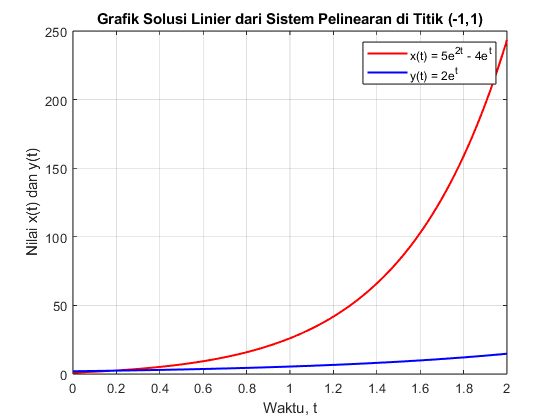
\includegraphics[width=0.45\textwidth]{1c.png}
                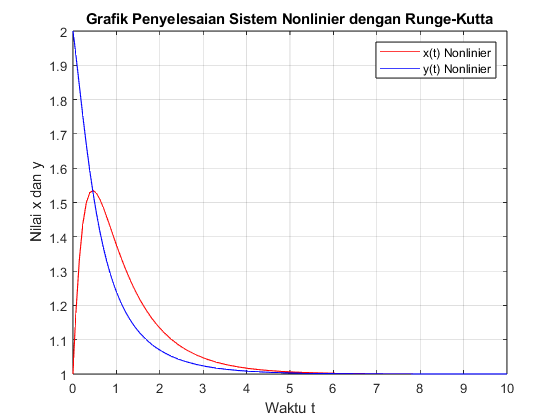
\includegraphics[width=0.45\textwidth]{1d.png}
            \end{figure}
        \end{enumerate}
        \item 
        \begin{enumerate}[label=\alph*.]
            \item Karena telah diketahui nilai ketika $t=0$, maka kita tinjau titik stabilitas non-negatif di $t=0$. Sehingga kita dapatkan:
            \begin{align*}
                4y - x^2 =0\\
                x - xy + 1=0
            \end{align*}
            Dengan mensubstitusi $y=\frac{x^2}{4}$ ke persamaan kedua, kita dapatkan:
            \begin{align*}
                x - x\left(\frac{x^2}{4}\right) + 1 &= 0\\
                x - \frac{x^3}{4} + 1 &= 0\\
                4x - x^3 + 4 &= 0\\
                x^3 - 4x - 4 &= 0
            \end{align*}
            Dengan menggunakan metode numerik, didapatkan nilai $x=2.383$ dan $y=1.42$.\\
            Selanjutnya kita linierkan model tersebut dengan menghitung matriks Jacobian dari model tersebut:
            \begin{align*}
                J_{(x,y)} &= \begin{bmatrix}
                    \pdv{f_1}{x} & \pdv{f_1}{y}\\
                    \pdv{f_2}{x} & \pdv{f_2}{y}
                \end{bmatrix} = \begin{bmatrix}
                    -2x & 4\\
                    1-y & -x
                \end{bmatrix}
            \end{align*}
            \item Substitusi titik stabilitas non-negatif ke dalam $J_{(x,y)}$ kita dapatkan:
            \begin{align*}
                J_{(2.383,1.42)} &= \begin{bmatrix}
                    -4.766 & 4\\
                    -0.58 & -2.383
                \end{bmatrix}
            \end{align*}
            Dengan menghitung nilai eigenvalue dari matriks diatas, kita dapatkan nilai eigenvalue-nya adalah $\lambda_1=3.5745+0.5102i$ dan $\lambda_2=-3.5745-0.5012i$. Karena nilai real dari eigenvalue-nya negatif maka model tersebut stabil.

            \item \(\lambda_1 = -3.5745 + 0.5102i\) akan didapat
    \[
    \begin{bmatrix}
        -4.766 - (-3.5745 + 0.5102i) & 4 \\
        -0.42 & -2.383 - (-3.5745 + 0.5102i)
    \end{bmatrix}
    \begin{bmatrix}
        x \\
        y
    \end{bmatrix}
    = \begin{bmatrix}
        0 \\
        0
    \end{bmatrix}
    \]
    
    Dengan menggunakan bantuan Matlab akan didapat vektor eigen yaitu
    \[
    v_1 = \begin{bmatrix} 0.9513 \\ 0.2834 + 0.1213i \end{bmatrix} \quad \text{dan} \quad v_2 = \begin{bmatrix} 0.9513 \\ 0.2834 - 0.1213i \end{bmatrix}
    \]
    
    \[
    U = e^{\lambda t} v_1
    \]
    
    \[
    U = e^{(-3.5745 + 0.5102i)t} \begin{bmatrix} 0.9513 \\ 0.2834 + 0.1213i \end{bmatrix}
    \]
    
    \[
    U = e^{-3.5745t} \left[ \cos 0.5102t + i \sin 0.5102t \right] \begin{bmatrix} 0.9513 \\ 0.2834 + 0.1213i \end{bmatrix}
    \]
    
    \[
    U = e^{-3.5745t} \begin{bmatrix} 0.9513 (\cos 0.5102t) + i \cdot 0.9513 (\sin 0.5102t) \\ 0.2834 (\cos 0.5102t) - 0.1213 (\sin 0.5102t) + i (0.1213 (\cos 0.5102t) + 0.2834 (\sin 0.5102t)) \end{bmatrix}
    \]

    Penyelesaian Umum:
    \[
    \begin{bmatrix} x(t) \\ y(t) \end{bmatrix} = C_1 \operatorname{Real}(U) + C_2 \operatorname{Im}(U)
    \]
    
    \begin{align*}
        \begin{bmatrix} x(t) \\ y(t) \end{bmatrix} =& C_1e^{-3.5745t} \begin{bmatrix} 0.9513 (\cos 0.5102t) \\ 0.2834 (\cos 0.5102t) - 0.1213 (\sin 0.5102t) \end{bmatrix} \\
        &+ C_2 e^{-3.5745t}\begin{bmatrix} 0.9513 (\sin 0.5102t) \\ 0.1213 (\cos 0.5102t) + 0.2834 (\sin 0.5102t) \end{bmatrix} 
    \end{align*}

    Penyelesaian Khusus:

    Dengan syarat awal : \( x(0) = 2 \) dan \( y(0) = 2 \), maka
    \begin{align*}
        \begin{bmatrix} x(0) \\ y(0) \end{bmatrix} &= C_1 e^{-3.5745(0)} \begin{bmatrix} 0.9513 (\cos 0.5102(0)) \\ 0.2834 (\cos 0.5102(0)) - 0.1213 (\sin 0.5102(0)) \end{bmatrix} \\
        &+ C_2 e^{-3.5745(0)} \begin{bmatrix} 0.9513 (\sin 0.5102(0)) \\ 0.1213 (\cos 0.5102(0)) + 0.2834 (\sin 0.5102(0)) \end{bmatrix}
    \end{align*}

Dari persamaan didapat \( C_1 = \frac{2}{0.9513} = 2.10 \) dan

\[
2.10 (0.2834) + 0.1213 C_2 = 2 \Rightarrow 0.1213 C_2 = 2 - 0.59514 = 1.40486
\]

\[
C_2 = \frac{1.40486}{0.1213} = 0.001
\]

Sehingga didapat \( C_2 = 0.001 \).

Oleh karena itu penyelesaian khusus persamaan adalah

\begin{align*}
\begin{bmatrix} x(t) \\ y(t) \end{bmatrix} =& 2.10e^{-3.5745t}\begin{bmatrix} 0.9513 (\cos 0.5102t) \\ 0.2834 (\cos 0.5102t) - 0.1213 (\sin 0.5102t) \end{bmatrix} \\+ 
&0.001e^{-3.5745t} \begin{bmatrix} 0.9513 (\sin 0.5102t) \\ 0.1213 (\cos 0.5102t) + 0.2834 (\sin 0.5102t) \end{bmatrix} 
\end{align*}
            \item Dengan cara yang sama seperti soal sebelumnya, kita dapatkan nilai-nilai yang diperlukan untuk menyelesaikan persamaan nonlinier secara numerik. Definisikan fungsi \( f(x,y) \) dan \( g(x,y) \) sebagai berikut:
            \begin{align*}
                f(x,y) &= 4y - x^2 + 2t\\
                g(x,y) &= x - xy + e^{2t}
            \end{align*}
            Dengan formula Runge-Kutta Orde 4, kita dapatkan:
            \begin{align*}
                k_{1x} &= 0.1 \cdot f(2,2) = 0.1 \cdot (8-4+0) = 0.4\\
                k_{1y} &= 0.1 \cdot g(2,2) = 0.1 \cdot (2-4+1) = -0.1\\
                k_{2x} &= 0.1 \cdot f\left(2 + \frac{0.4}{2}, 2 + \frac{-0.1}{2}\right) = 0.1 \cdot f(2.2,1.95) = 0.1 \cdot (8-4.84+0.2) = 0.326\\
                k_{2y} &= 0.1 \cdot g\left(2 + \frac{0.4}{2}, 2 + \frac{-0.1}{2}\right) = 0.1 \cdot g(2.2,1.95) = 0.1 \cdot (2-4.4+1) = -0.1\\
                k_{3x} &= 0.1 \cdot f\left(2 + \frac{0.363}{2}, 2 + \frac{-0.1}{2}\right) = 0.1 \cdot f(2.1815,1.95) = 0.1 \cdot (8-4.75+0.21815) = 0.342\\
                k_{3y} &= 0.1 \cdot g\left(2 + \frac{0.363}{2}, 2 + \frac{-0.1}{2}\right) = 0.1 \cdot g(2.1815,1.95) = 0.1 \cdot (2-4.363+1) = -0.1\\
                k_{4x} &= 0.1 \cdot f(2.2425,1.95) = 0.1 \cdot (8-5.03+0.2425) = 0.271\\
                k_{4y} &= 0.1 \cdot g(2.2425,1.95) = 0.1 \cdot (2-4.485+1) = -0.1
            \end{align*}
            Misalkan kita ingin mencari nilai $x(0.1)$ dan $y(0.1)$, maka kita dapatkan:
            \begin{align*}
                x(0.1) &= 2 + \frac{1}{6}(0.4 + 2(0.326) + 2(0.342) + 0.271) = 2.2425\\
                y(0.1) &= 2 + \frac{1}{6}(-0.1 + 2(-0.1) + 2(-0.1) - 0.1) = 1.95
            \end{align*}
            Untuk nilai $t$ yang lain dapat dicari menggunakan rumus iteratif yang telah disebutkan diatas.
            \item Berikut adalah grafik penyelesaian dari poin (c) dan (d) menggunakan MATLAB:
            \begin{figure}[h!]
                \centering
                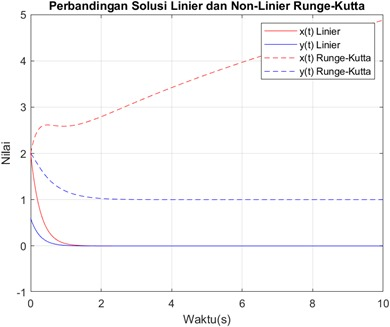
\includegraphics[width=0.5\textwidth]{2cd.jpg}
            \end{figure}
        \end{enumerate}
    \end{enumerate}
        
\end{document}